\chapter{這本講義怎麼做出來的 \\ \LaTeX 教學}
\chapterauthor{李杰穎}
\setcounter{section}{-1}
\section{前言}
Hi各位,我是編這本講義的熊熊,大家有沒有發現這本講義好像不是用Word打出來的,很多地方都跟Word不太一樣。\\
其實這本講義是由\LaTeX 打出來的喔。
\section{蛤,\LaTeX 是甚麼}
{\Kai \LaTeX 是一種基於是一種基於TeX的排版系統,由美國電腦科學家萊斯利·蘭伯特在20世紀80年代初期開發,利用這種格式系統的處理,即使使用者沒有排版和程式設計的知識也可以充分發揮由TeX所提供的強大功能,不必一一親自去設計或校對,能在幾天,甚至幾小時內生成很多具有書籍品質的印刷品。對於生成複雜表格和數學公式,這一點表現得尤為突出。因此它非常適用於生成高印刷品質的科技和數學、物理文件。這個系統同樣適用於生成從簡單的信件到完整書籍的所有其他種類的文件。}\\
\rightline{\textit{from wikipedia}} 

簡單來說,\LaTeX 算是一種寫文件的方法,不過這種方法與一般的文書軟體不同,並不是所見即所得(What You See Is What You Get;WYSIWYG),而是一種類似透過寫程式語言的方法來完成,然後再經過xelatex這種類似程式語言編譯器的``排版引擎"編譯出pdf檔,來生成你們現在看到的文字、數學式、圖片...
\begin{figure}[H]
    \centering
    \graphicspath{{informatics/}}
    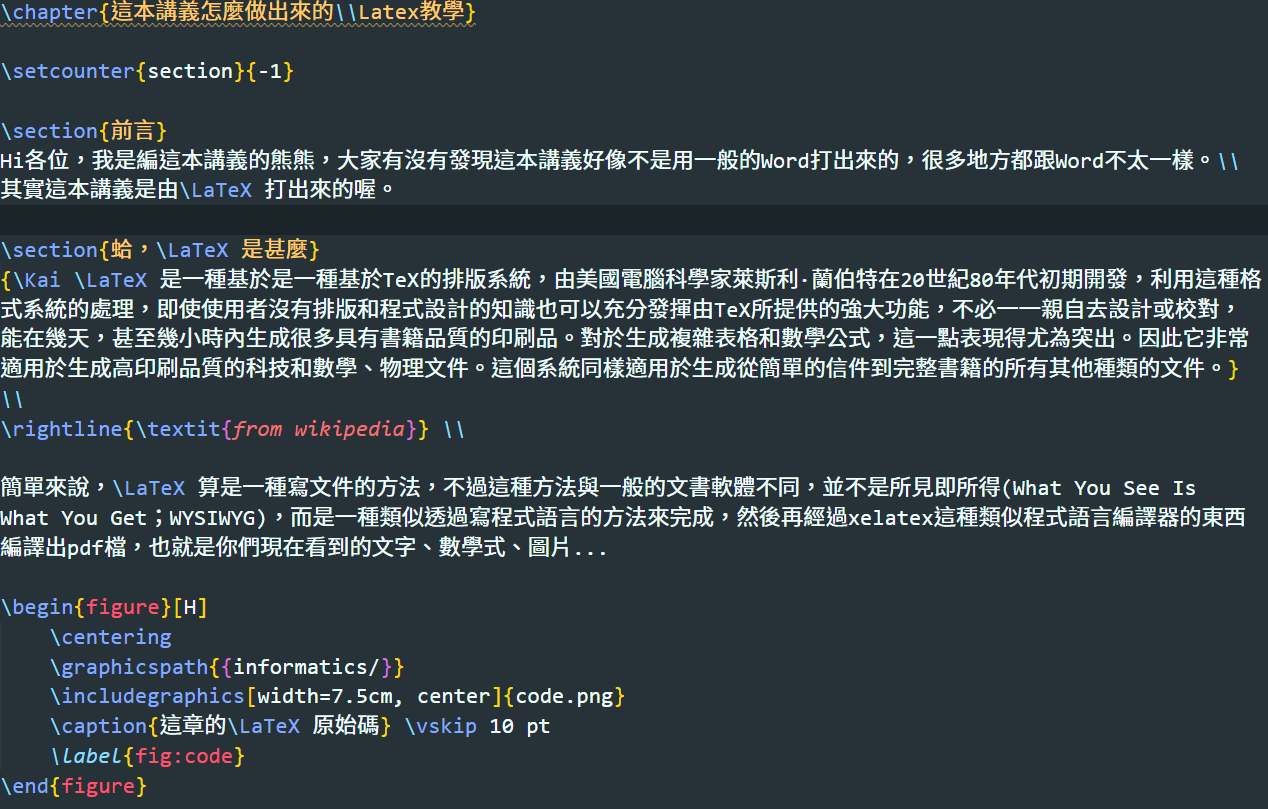
\includegraphics[width=5cm, center]{code.png}
    \caption{這章的\LaTeX 原始碼} \vskip 10 pt
    \label{fig:code}
\end{figure}

\section{用\LaTeX 有甚麼好處}
當你使用\LaTeX 來編寫文件、書籍、論文等等...,你不用像Word一樣一直管排版,也不用一直管圖片到底要放在哪裡,大小要多大之類的,你只要專心在你文件的內容,變相提升你的效率。

而且它還可以自動生成目錄,自動生成章節、圖片的編號,相當的強大。

但是它的安裝及文件的版面設定非常不友善,跟Word這種幾乎不用什麼設定的軟體差的非常多,這是\LaTeX 的致命傷之一。

\begin{figure}[H]
    \centering
    \graphicspath{{informatics/}}
    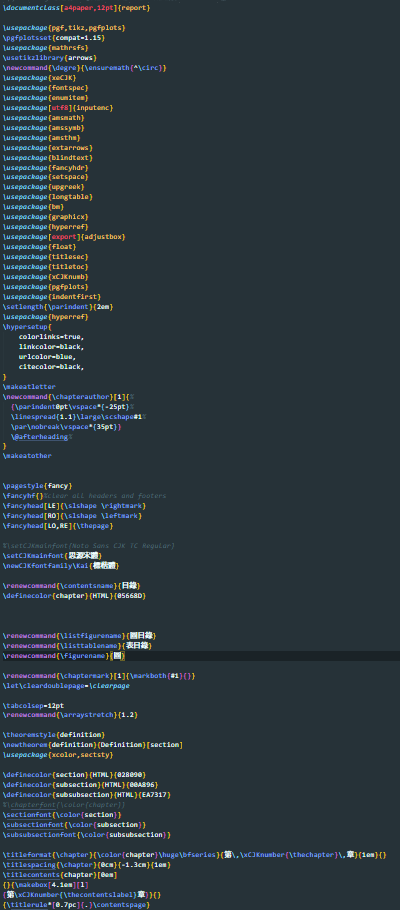
\includegraphics[width=5cm, center]{setting.png}
    \caption{這本講義的前置設定} \vskip 10 pt
    \label{fig:setting}
\end{figure}

\section{\LaTeX 安裝教學}
我這邊有打一份\LaTeX 的安裝教學,對使用\LaTeX 的編寫及使用有興趣的人可以去下面的網址看看。 \\
\url{http://bit.ly/latex-installation}

\section{講師介紹}
\begin{itemize}
\item 姓名:李杰穎
\item 性別:公熊
\item 特色:為班上的存在王,喜愛裝弱和否認自己裝弱,再接著說自己真的很弱。因為戀愛不順常常收好人卡(編按:對熊熊說你是個好人,就會有意料之外的事情喔!),因此埋首在電腦的世界中,是資訊電神喔!他擅長同意別人的說法,和說尷尬笑話,也擅長同意別人說尷尬笑話,所以要說笑話可以去找熊熊喔!
\item 名言:完了、喔不、我是廢物(單邊嘴唇)、你看麻這這這是這樣麻對不對不是麻你看就是是是這樣阿
\end{itemize}